\documentclass[11pt,a4paper]{article}
\usepackage[latin1]{inputenc}
\usepackage{amsmath}
\usepackage{amsfonts}
\usepackage{amssymb}
\usepackage{booktabs}
\usepackage{graphicx}
\usepackage{wrapfig}
\usepackage{sidecap}
\usepackage{subfig}
\usepackage{longtable}
\usepackage{listings}
\lstset{
frame=single,	                % adds a frame around the code
tabsize=4,	                % sets default tabsize to 2 spaces
captionpos=b,                   % sets the caption-position to bottom
breaklines=true,                % sets automatic line breaking
breakatwhitespace=false        % sets if automatic breaks should only happen at whitespace
}


\author{Wouter ibens}
\title{Lindenmayer Systems, an efficient implementation}

\newcommand{\degree}{\ensuremath{^\circ}} 
\begin{document}
\maketitle
\tableofcontents
\newpage
\section{What are L-Systems}
L-systems or Lindenmayer systems are a way of visualizing any kind of abstract object. It is most often used for fractals and plants or flowers, but variants exist for DNA representation, bit errors in data streams and many more.

\subsection{Turtle Graphics}
Lindenmayer systems rely on turtle graphics as drawing technique. It specifies a turtle or pen, which has a position, a direction and an specified angle $\sigma$. This pen can draw forward, move forward and turn left or right over $\sigma$. Drawing results in a line of length 1 and an updated position, where moving only results in the latter. Turning only results in an updated direction.
To control the pen, a set of commands is given as an input string. Where each symbol represents a command.
\begin{center}
\begin{tabular}{c | l}
Symbol & Action \\ \hline
F & Draw forward \\
f & Move forward \\
+ & Turn left over $\sigma$ \\
- & Turn right over $\sigma$
\end{tabular}
\end{center}

So the string F+F+F+F and $\sigma = 90\degree$ would result in a square. A more complicated example is the Koch curve given in figure \ref{fig:koch}.
\begin{figure}[h!]
  \centering
  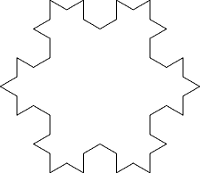
\includegraphics[]{koch.png}
  \caption{Koch curve drawn using turtle graphics}
  \label{fig:koch}
\end{figure}

\subsection{Lindenmayer Systems}
L-Systems use formal grammar techniques to extend the possibilities of turtle graphics in a way fractals are easier producible. An L-System is given an axiom and a set of rules $X \rightarrow Y$ where $X$ is a character in the alphabet and $Y$ is a string of characters in the alphabet. Except for fractals, L-Systems are very often used to generate plants and trees. The Koch curve in figure \ref{fig:koch} can be given as an L-System.

\begin{table}
\center
\begin{tabular}{l l}
Axiom & $F--F--F$ \\ \hline
$\sigma$ & 60\degree \\ \hline
Rules & $F \rightarrow F+F--F+F$ \\
\end{tabular}
\caption{The Koch-curve as an L-System}
\end{table}

\begin{figure}[h]
  \centering
  \subfloat[][Axiom]{\label{fig:koch1}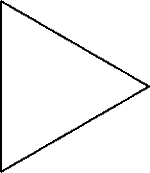
\includegraphics[width=0.23\textwidth]{koch1.png}}
  \hspace{0.01\textwidth}
  \subfloat[][First Iteration]{\label{fig:koch2}
\includegraphics[width=0.23\textwidth]{koch2.png}}
  \hspace{0.01\textwidth}
  \subfloat[][Second Iteration]{\label{fig:koch3}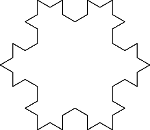
\includegraphics[width=0.23\textwidth]{koch3.png}}
  \hspace{0.01\textwidth}
  \subfloat[][Third Iteration]{\label{fig:koch4}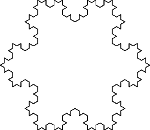
\includegraphics[width=0.23\textwidth]{koch4.png}}
  \caption{Iterating the Koch curve}
  \label{fig:animals}
\end{figure}


\begin{figure}[h!]
  \centering
  
\includegraphics[]{dragon.png}
  \caption{Dragon curve}
  \label{fig:dragon}
\end{figure}

The first iteration of an L-System is done by substituting the symbols in the axiom with the body of respectively production rule. The following steps use the resulting string of the previous step as axiom.

\subsection{Extensions}
Although this basic set of commands allows us to draw some nice pictures, many extensions have been added to maximize the possibilities of L-Systems. The implemented extensions are given in this subsection.

\subsubsection{Brackets}
Brackets are used to save the current state (at least the current position and direction) to a stack. This allows us to start a subexpression as new branch, but return later on to the original position and continue its root branch.

\begin{center}
\begin{tabular}{c | l}
Symbol & Action \\ \hline
[ & Push the current state to the stack \\
] & Pop the last saved state from the stack \\
\end{tabular}
\end{center}

\begin{figure}[htb]
  \centering
  \begin{minipage}[c]{0.65\textwidth}
    \centering
    \begin{tabular}{l l}
Axiom & $X$ \\ \hline
$\sigma$ & $22.5$\degree \\ \hline
Rules & $X \rightarrow F-[[X]+X]+F[+FX]-X$ \\
& $F \rightarrow FF$ \\
	\end{tabular}
  \end{minipage}
  \begin{minipage}[c]{0.33\textwidth}
    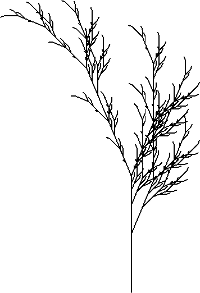
\includegraphics[width=\textwidth]{tree.png}
  \end{minipage}
  \caption{Simple 2D plant with brackets}
  \label{fig:tree}
\end{figure}

\subsubsection{3D}
To create more realistic models of objects, 3D was introduced. Instead of just turning left and right, it gives support for rotating the pen and adjust its pitch.

\begin{center}
\begin{tabular}{c | l}
Symbol & Action \\ \hline
\& & Pitch down \\
\^{} & Pitch up \\
/ & Roll right \\
$\backslash$ & Roll left \\
$\vert$  & Turn 180\degree \\
\end{tabular}
\end{center}

\begin{figure}[htb]
  \centering
  \begin{minipage}[c]{0.65\textwidth}
    \centering
    \begin{tabular}{l l}
Axiom & $F$ \\ \hline
$\sigma$ & $28$\degree \\ \hline
Rules & $F \rightarrow F[\&+F]F[-\backslash F][\&F]$
	\end{tabular}
  \end{minipage}
  \begin{minipage}[c]{0.25\textwidth}
    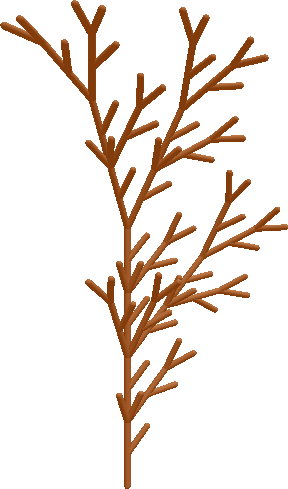
\includegraphics[width=\textwidth]{3dtree.png}
  \end{minipage}
  \caption{A 3D plant}
  \label{fig:3dtree}
\end{figure}

\subsubsection{Polygons}
To improve the realism of the models even more, flowers and leaves should be added to them. Therefore polygons should be supported by the system. A polygon is similar to the stack as it also stores a position (B) on the stack. When a polygon is started every position the pen moves to will create a new triangle. The corners of this triangle are the top of stack (B), the point it just moved to, and the previous position. Obviously, after the first movement the top of stack and the previous position are the same so no triangle will be created. To support this settings the state of the pen must be extended with a polygon mode, which must be set to true when we want to start a new polygon. Figure \ref{fig:polygon} is the visualization of the following string ($\sigma = 30\degree$):
\begin{verbatim}
F{-f+f+f-|-f+f+f}
\end{verbatim}


\begin{figure}[h!]
  \centering
  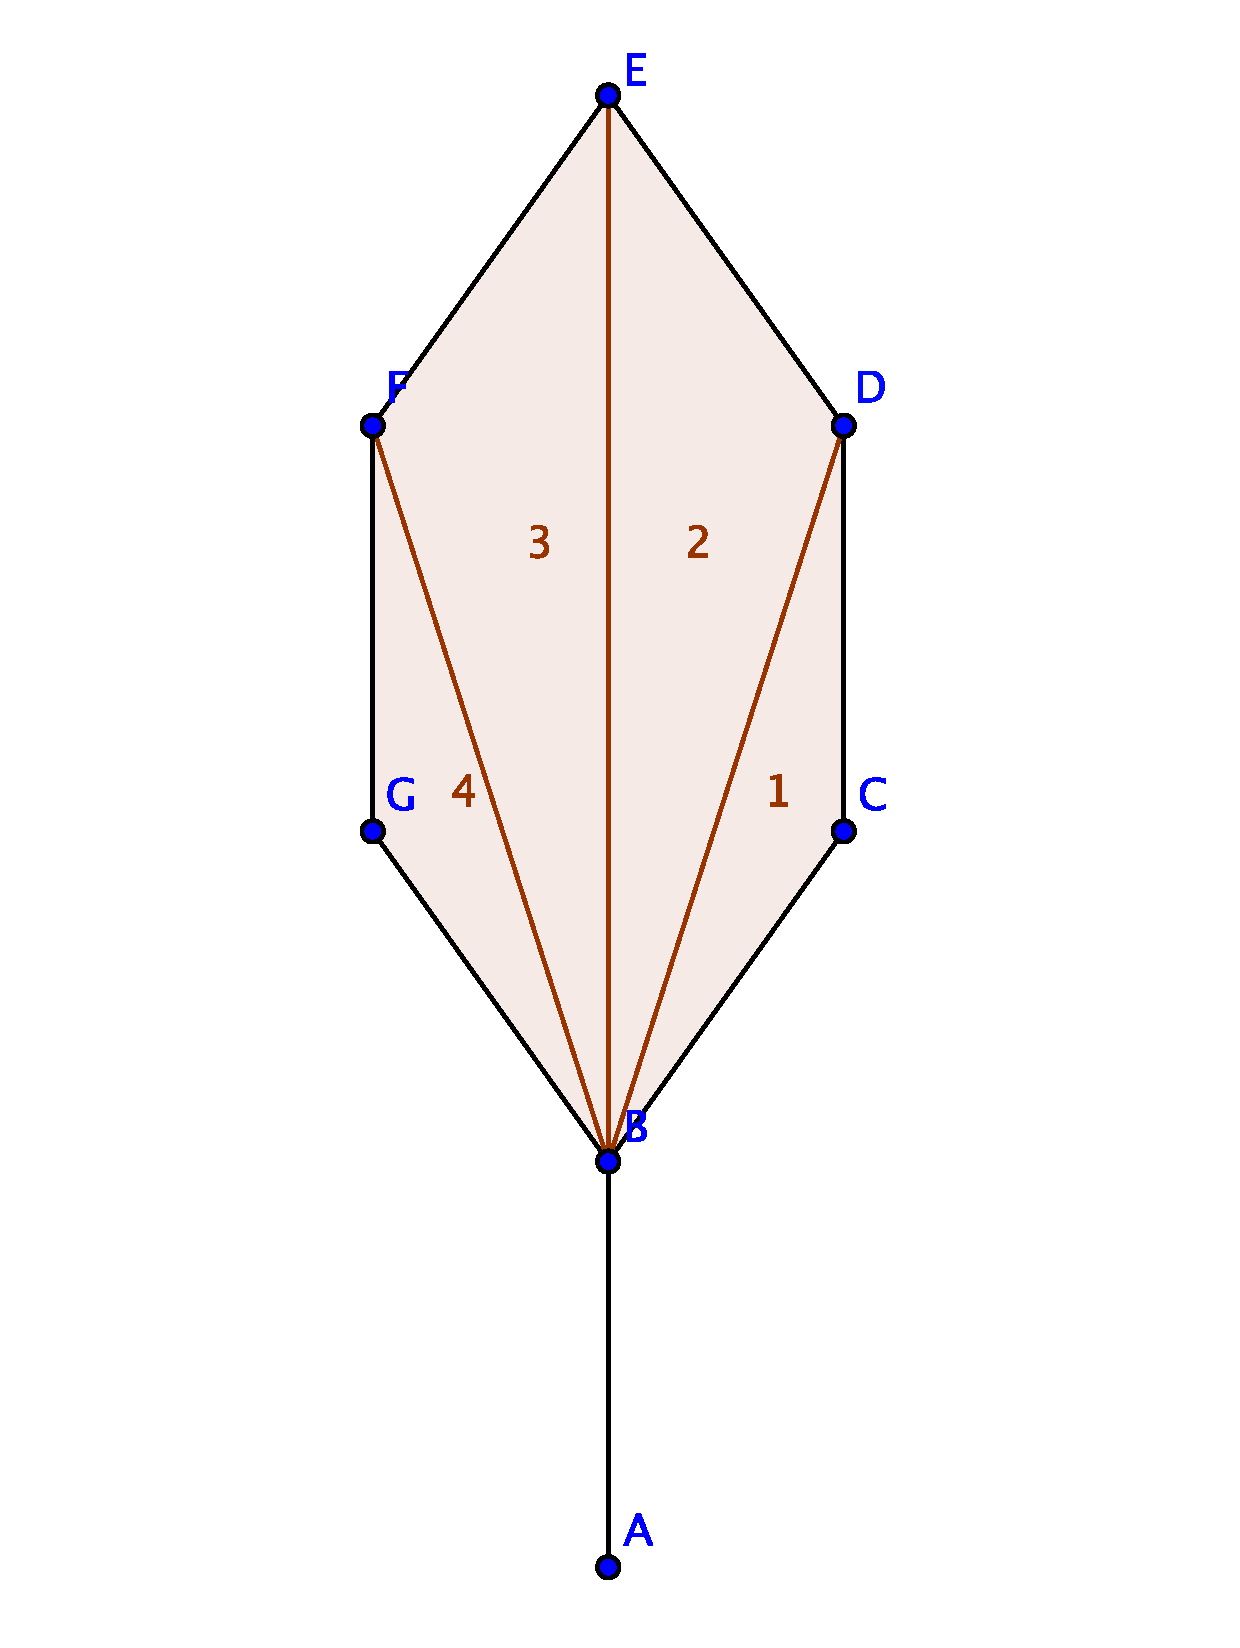
\includegraphics[width=0.35\textwidth]{polygons.pdf}
  \caption{How a polygon is drawn}
  \label{fig:polygon}
\end{figure}

\begin{center}
\begin{tabular}{c | l}
Symbol & Action \\ \hline
\{ & Push the current state to the stack and set polygon mode \\
\} & Pop the last saved state from the stack \\
\end{tabular}
\end{center}

%\begin{figure}[h!]
%  \centering
%  
\includegraphics[width=0.25\textwidth]{polys.png}
%  \caption{Example of polygons: lily}
%  \label{fig:polyexample}
%\end{figure}

\subsubsection{Pen style}
Another extension is the pen style, this includes both line length and thickness as the color. Default, an L-System starts with a line length of 1 and 10\% of the length as thickness. This allows us to draw a thick trunk and smaller branches, or brown trees with green leaves. The pen style is also part of the state, so it gets saved whenever we push the stack.

\begin{center}
\begin{tabular}{c | l}
Symbol & Action \\ \hline
! & Reduce thickness by 30\% \\
? & Increase thickness by 40\% \\
' & Reduce length by 10\% \\
" & Increase length by 10\% \\
c & Increase color index by 1
\end{tabular}
\end{center}


\subsubsection{Parameters}
The last implemented extension is the ability to give each command and optional parameter, specified between brackets after the command it applies to. Using parameters makes it possible to turn by an angle, other than $\sigma$ or specify a fixed color constant.

\begin{figure}[h]
  \centering
  \subfloat[][Lily]{\label{fig:lilypov}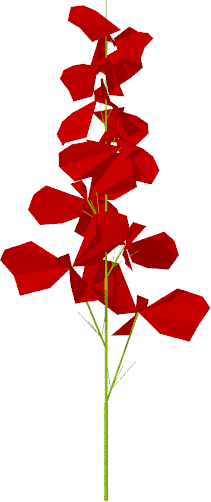
\includegraphics[width=0.27\textwidth]{lily_red.png}}                
  \subfloat[][Plant]{\label{fig:treepov}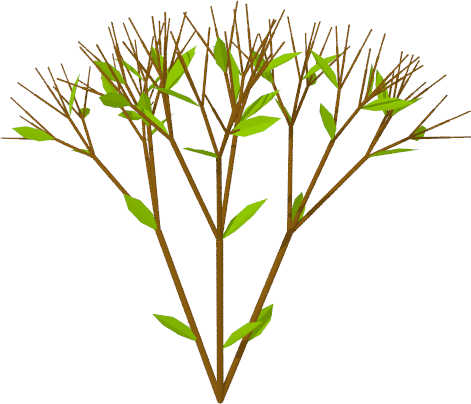
\includegraphics[width=0.73\textwidth]{plant6.png}}
  \caption{POVRay renders of L-Systems}
  \label{fig:povrenders}
\end{figure}

\begin{center}
\begin{longtable}{l | l}
Symbol & Action \\ \hline
F & Draw a line of 1 unit \\
F(x) & Draw a line of x units \\
f & Move forward by 1 unit \\
f(x) & Move forward by x units \\
Z & Draw a line of half a unit \\
Z (x) & Draw a line x/2 units \\
z & Move half a unit \\
z(x) & Move by x/2 units \\
+ & Turn left over $\sigma$ \\
+(x) & Turn left over x\degree \\
- & Turn right over $\sigma$ \\
-(x) & Turn right over x\degree \\
$[$ & Push the current state to the stack \\
$]$ & Pop the last saved state from the stack \\
\& & Pitch down over $\sigma$ \\
\&(x) & Pitch down over x\degree \\
\^{} & Pitch up over $\sigma$ \\
\^{}(x) & Pitch up over x\degree \\
/ & Roll right over $\sigma$ \\
/(x) & Roll right over x\degree \\
$\backslash$ & Roll left over $\sigma$ \\
$\backslash$(x) & Roll left over x\degree \\
$\vert$  & Turn 180\degree \\
\{ & Push the current state to the stack and set polygon mode \\
\} & Pop the last saved state from the stack \\
! & Reduce thickness by 30\% \\
? & Increase thickness by 40\% \\
!(x),?(x) & Thickness = thickness * x \\
' & Reduce length by 10\% \\
" & Increase length by 10\% \\
'(x),"(x) & Length = length * x \\
c & Increase color index by 1 \\
c(x) & Set color index to x \\
\end{longtable}
\end{center}

\subsection{Efficiency} % both time and space approach and complexity
Implementing a program to calculate and draw Lindenmayer systems is not a big challenge. There is a very naive way of doing this, which will be explained later on, but this method is in general very slow and consumes huge amounts of memory. We will try to speed things up by implementing a more complex data structure and using some general optimizations. The approach of this project was to minimize both time and space complexity.

\newpage
\section{Implementation}

A Lindenmayer system in a datastructure always consists of:
\begin{enumerate}
\item An alphabet \label{structalpha}
\item An axiom, a string \label{structaxiom}
\item A list of production rules, a pair (character, string) \label{structrules}
\item A default angle $\sigma$, a double for the radial of degree representation
\item A dictionary, telling what characters cause what action
\item Optionally a set of colors
\end{enumerate}
Only \ref{structalpha}, \ref{structaxiom} and \ref{structrules} are required for the string production. And since the alphabet is usually the machines character set, there is no need to store this in the program.

\subsection{String iteration, the naive approach}

Iterating L-systems is not very difficult using string iteration. Your program only needs the production rules and the axiom, no preprocessing is required. From the previous step or axiom, the program loops over every character and adds the substitution of that character to the new string or the character itself if no production rule is found.

\lstset{label=code:stringit,caption=String iteration}
\begin{lstlisting}
//Given: axiom (string), rules (array of string)
currentstring = axiom
iteration = 0

function iterate()
	newstring = ""
	iteration = iteration + 1
	foreach c in currentstring
		if (c in rules)
			newstring = newstring + rules[c]
		else
			newstring = newstring + c
	currentstring = newstring
\end{lstlisting}

The code \ref{code:stringit} shows the algorithm to iterate currentstring to the next iteration. This is a fairly easy implementation of both the algorithm and the datastructure but has some huge disadvantages: iterating the L-system found in \ref{fig:3dtree} 12 times returns a string of size 915527344 (~873 MB). Besides the memory usage, it took tens of minutes to process the last 3 iterations. Anoter small disadvantage is the fact you cannot go back one iteration without recalculating it from the axiom to that iteration.

\subsection{A more efficient data structure} %and maybe the draw inside the calc

The only production rule in \ref{fig:3dtree} is $F \rightarrow F[\&+F]F[-\backslash F][\&F]$.

\subsection{See the difference} %benchmark results

\section{Stochastic L-Systems} %and how is fucks the datastructure
\subsection{Implementation}
\subsection{Memory usage}

\section{Brighten things up} % features, rounding, GUI, ...

\section{Efficiency tricks}

\section{Conclusion}

\newpage
\begin{appendix}
\listoffigures
\end{appendix}
\end{document}